%%%%%%%%% PROJECT DESCRIPTION  -- 15 pages (including Prior NSF Support)

\required{Project Description}
\begin{center}
%\emph{Maximum of 15 pages}
\end{center}
%The Project Description (including Results from Prior NSF Support, which is
%limited to five pages) may not exceed 15 pages. Visual materials, including charts,
%graphs, maps, photographs and other pictorial presentations are included in the
%15-page limitation. PIs be cautioned that the project description must
%be self-contained and that URLs that provide information related to the proposal
%should not be used. \\
%
%All proposals to NSF are reviewed utilizing the two merit review criteria,
%intellectual merit and broader impacts. \\
%
% The Project Description should provide a clear statement of the work 
% to be undertaken and must include: objectives for the period of the proposed 
% work and expected significance; relation to longer-term goals of the PI's 
% project; and relation to the present state of knowledge in the field, 
% to work in progress by the PI under other support and to work in progress 
% elsewhere.

%%%%%%%%%%%%%%%%%%%%%%%%%%%%%%%%%%%%%%%%%%%%%%%%%%%%%%%%%%%%%%%%%%%%%%
%INTRO
%%%%%%%%%%%%%%%%%%%%%%%%%%%%%%%%%%%%%%%%%%%%%%%%%%%%%%%%%%%%%%%%%%%%%%
\section*{Introduction}

While the potential role of hybridization and introgression as agents of evolution has long been postulated \citep{Anderson1948, Anderson1954, Stebbins1959}, only recently have technological innovations allowed for characterization of these processes on a genome-wide scale. 
Multiple studies have now reported evidence of inter-taxon introgression in both plant \citep{Hufford2013, renaut2013} and animal \citep{consortiumbutterfly2012, staubach2012, huerta2014} species based on full-genome data.
Genomic tools provide the capacity to evaluate the genomic extent of introgression, differentiate neutral from adaptive introgression, and evaluate whether distinct hybrid populations show convergent patterns of introgression.
With this expanded perspective, we can fully evaluate hypotheses first articulated by \citet{Anderson1954}: that 1) Evolution can occur rapidly through selection on novel variation generated by hybridization, and 2) The shuffling and redistribution of previously isolated species through anthropogenic activity has provided ample opportunity for hybridization to occur \citep{Anderson1954}.
Given its evolutionary history and genomic resources, the \emph{Zea} study system represents an unparalleled opportunity for testing these hypotheses and realizing the promise of genomic data for hybridization studies.

In the investigation proposed here, we will build upon our previous work in maize (\emph{Zea mays} ssp. \emph{mays}) and its wild relatives the teosintes (\emph{Zea} spp.) to characterize the evolutionary role of hybridization and introgression in this system. 
First, analysis of hybridization in two parapatric and uniquely-adapted teosinte subspecies will allow us to answer questions about convergent introgression and the extent to which selection determines patterns of gene flow.
Second, evaluation of introgression between maize and teosinte outside the domestication center will inform our understanding of the importance of adaptive introgression during colonization of novel environments and test the role of widespread species to act as bridges for gene flow among their congeners.

This proposal builds considerably upon a previous full submission to the 2014 NSF-DEB competition that was favorably reviewed but not funded due to concerns over certain aspects of experimental design that we have rectified here.
In addition, over the last year we have conducted additional preliminary analyses, solidified collaborations with colleagues in Mexico and Guatemala, and ensured that this project is logistically feasible.

%%%%%%%%%%%%%%%%%%%%%%%%%%%%%%%%%%%%%%%%%%%%%%%%%%%%%%%%%%%%%%%%%%%%%%
%OBJECTIVES
%%%%%%%%%%%%%%%%%%%%%%%%%%%%%%%%%%%%%%%%%%%%%%%%%%%%%%%%%%%%%%%%%%%%%%
\section*{Objectives}
\jri{make sure these are in same order with same wording as below!}
\subsection*{Objective I: Assess the evolutionary role of hybridization in a naturally occurring teosinte hybrid zone}
\emph{Zea mays} ssp. \emph{parviglumis} (the wild progenitor of maize; hereafter, \zp) and \emph{Zea mays} ssp. \emph{mexicana} (hereafter, \emph{mexicana}) diverged approximately 60,000 BP \citep{Ross-Ibarra2009a} and have parapatric distributions: while \zp\ occurs in the warm lowlands of southwest Mexico, \zm\  is found in the cool highlands of the Central Plateau. 
Narrow regions of admixture between these wild subspecies have been discovered at middle elevations \citep{Fukunaga2005, Pyhajarvi2013}. 
Through targeted collections, high-density genotyping, population genomic analyses, and common garden experiments, we will address the following research questions: 

\begin{enumerate}
\item \emph{Do hybrid populations show higher fitness than parental subspecies in some environments?}
\item \emph{Is there evidence of selection on putatively adaptive phenotypes across hybrid zones?}
\item \emph{Do independent hybrid zones show convergent or unique patterns of introgression?}
\end{enumerate}

\subsection*{Objective II: Determine the extent to which anthropogenic movement of maize has enabled hybridization among taxa in \emph{Zea}}
Maize was domesticated in southwest Mexico from \zp{} $\sim$9,000 BP \citep{Matsuoka2002} and quickly spread throughout the Americas, bringing it into contact with other teosinte taxa.
Hybridization has been observed between maize and each of these teosintes, raising questions about the interaction between colonization and hybridization. \jri{never sure when to use ``gene flow'', ``introgression'', or ``hybridization''. could you make sure we are using appropriately and consistently throughout?}
Our population genetic analysis will assess the following questions:
\begin{enumerate}
\item \emph{Is introgression adaptive across multiple geographic scales?}
\item \emph{Does hybridization with locally-adapted relatives facilitate the spread of colonizing species?}
\item \emph{Can a widespread species serve as a bridge for gene flow among otherwise allopatric taxa?} 
\end{enumerate}

%%%%%%%%%%%%%%%%%%%%%%%%%%%%%%%%%%%%%%%%%%%%%%%%%%%%%%%%%%%%%%%%%%%%%%
%RATIONALE AND SIGNIFICANCE
%%%%%%%%%%%%%%%%%%%%%%%%%%%%%%%%%%%%%%%%%%%%%%%%%%%%%%%%%%%%%%%%%%%%%%
\section*{Rationale and Significance} 
\jri{no figures in first 4 pages. think this is a problem?}
Pioneers in evolutionary biology including G. Ledyard Stebbins and Edgar Anderson recognized the important role hybridization and introgression could play in adaptation and speciation \citep{Anderson1948, Anderson1954}.
These evolutionary forces were thought to be particularly influential when environmental conditions encountered by a species were marginal, variable, or new \citep{Stebbins1959}.
More recently, defined and stable regions of hybridization, referred to as hybrid zones, have been discovered in a number of taxa \citep[reviewed in ][]{HarrisonHybridZone, shurtliff2013, abbott2014}. 
It is increasingly clear that the phenomena of hybridization and subsequent introgression shape genomes and influence the trajectory of species as they evolve \citep{Ellstrand2014}.
Hybridization has long been believed to play a role in speciation, and introgression of even a small number of loci can enable a species to adapt and invade novel habitats \citep{currat2008, abbott2013}.
For example, we now have strong molecular evidence that hybridization has led to speciation in both plants and animals \citep[reviewed in][]{mallet2007} and that colonization events of non-native species \citep{lucek2010} and domesticated crops \citep{he2011, Hufford2013} have been facilitated by introgression. 

While theory regarding hybridization has progressed and many compelling empirical examples have been identified, several outstanding questions remain. 
For example, are hybrid zones maintained by adaptive or purifying selection or strictly neutral processes \citep{Kruuk1999, Rasmussen2012, Smith2013b}? 
If introgression is adaptive, what is the geographic scale of this adaptation?
Are the same adaptive alleles introgressed across independent hybrid populations or are patterns of introgression driven more by local environmental conditions?
Can a widespread congener act as a bridge for gene flow between more narrowly distributed allopatric taxa? \jri{do we want these to perfectly mirror objectives?}
Genome-wide analysis of variation in the extent and genetic architecture of introgression --- the number and size of introgressed loci ---  will offer considerable insight regarding each of these questions.  
For example, the few genomic studies of introgression completed thus far have already suggested that rates of gene flow vary substantially across loci, likely as a function of selection on introgressed alleles \citep{Hufford2013, Poelstra2014}, and that introgression has occurred at genomic locations underlying adaptive phenotypes that may have facilitated colonization of a non-native taxon \citep{Hufford2013}.\jri{do we need more broad-scale big picture stuff? this section very quickly jumps into maize details. maybe cite \citep{rieseberg2007hybridization} somewhere too}
 


%%%%%%%%%%%%%%%%%%%%%%%%%%%%%%%%%%%%%%%%%%%%%%%%%%%%%%%%%%%%%%%%%%%%%%
%SPECIFIC OBJECTIVES
%%%%%%%%%%%%%%%%%%%%%%%%%%%%%%%%%%%%%%%%%%%%%%%%%%%%%%%%%%%%%%%%%%%%%%
\section*{Research Plan}

\jri{see commented text here for outline for objectives}

%\subsection{OBJECTIVE}
%background paragraph on relevant biology
%\subsubsection{A}
%paragraph describing hypotheses and predictions
%paragraphs explaining what we're gonna do
%\subsubsection{B}
%paragraph describing hypotheses and predictions
%paragraphs explaining what we're gonna do
%\subsubsection{C}
%paragraph describing hypotheses and predictions
%paragraphs explaining what we're gonna do
%\subsubsection{Prelim Results}
%What data we have so far
%\subsubsection{Potential Challenges}
%not interpretation of hypotheses but explicitly what if something goes wrong what we do.


\subsection{Assess the evolutionary role of hybridization in a naturally ocurrring teosinte hybrid zone}
\label{ss:hybrids}

\jri{paragraphs on background here}
The \emph{Zea} study system is uniquely suited to address these questions and advance our understanding of the hybridization biology.
The \emph {Zea mays} subspecies \emph{parviglumis} and \emph{mexicana} are distributed across a steep altitudinal gradient and differ for phenotypes that are thought to be adaptive in the highlands such as the presence of macrohairs, stem pigmentation and shorter flowering time in \emph{mexicana}.
A recent ecological niche study has found that the potential distributions of these subspecies are largely allopatric and stable over many thousands of years \citep{hufford2012inferences}.
However, analysis of microsatellite markers genotyped in a range-wide sample has identified elevated admixture between the subspecies in two geographically-distinct, mid-elevation regions of Mexico where the distributions of parental subspecies overlap, suggesting the presence of multiple hybrid zones \citep{Fukunaga2005}.  
Our recent genome-wide analysis of twelve individuals from a population in one of these hybrid zones revealed abundant small blocks of admixture in all individuals, suggesting long-term gene flow between subspecies \citep{Pyhajarvi2013}.  
Very little is known, however, about patterns of introgression across populations in this region or in independent hybrid zones.
By expanding our preliminary studies beyond a single population, we can assess how introgression varies across regions and hybrid zones and determine if specific haplotypes are consistently introgressed and widely adaptive or, rather, tied to specific habitats. 


\subsubsection{Do hybrid populations show higher fitness than parental subspecies in some environments?} 
\label{sss:fitness}

\jri{paragraph on tension zone vs. ecoton hypotheses and predictions here}

In order to assess fitness and variation at putatively adaptive phenotypes across both non-admixed and  hybrid populations we will conduct common garden experiments in Mexico at three altitudes: 1) Below a hybrid zone in habitat occupied by non-admixed \emph{parviglumis}; 2) Within hybrid zone habitat; and 3) Above a hybrid zone in habitat occupied by non-admixed \emph{mexicana}. 
Common garden experiments will be replicated over years two and three of our proposed project.  

Discussions with collaborators in Mexico (Ruairidh Sawers and Salvador Montes-Hernandez; see attached letters of commitment) raised concerns about the safety of students at field sites in the state of Guerrero (the location of the eastern Balsas hybrid zone; see US State Department Travel Warning at \url{http://travel.state.gov/content/passports/english/alertswarnings/mexico-travel-warning.html}) and the feasibility of managing six concurrent gardens. We thus propose a single transect of three replicate gardens in the eastern Jalisco hybrid zone. 
In our initial discussions with Drs. Sawers and Montes-Hernandez we have identified potential high- and low-elevation sites near Celaya and Bucerias, Mexico respectively.  
We will explore options for our third hybrid zone garden during our collections in the first year of the project.
The hybrid zone is less than 50 kilometers from the host institution of Dr. Sawers (Langebio in Irapuato, Mexico) and identification of an appropriate site should be straight-forward.
Each garden will consist of three complete blocks including a randomization of three plants from each of 15 sampling sites in the 16 populations described in \ref{sss:genomescan} (3 blocks x 3 plants x 15 sites x 16 populations = 2,160 plants per garden).  
We will measure fitness-related phenotypes (percent germination, germination rate, plant height at 15-day intervals, seed set, 50-seed weight, total-above-ground biomass, stomatal conductance and survival), putatively adaptive phenotypes across the altitudinal gradient (macrohair density, pigmentation extent, and flowering time) and phenotypes for which there is no \emph{a priori} evidence of selection across an elevational gradient (culm diameter \jri{culm diameter associated with Inv1n which shows altitudinal clines (Fang2012); wider in mex than parv; might show cline.} and the width of the leaf beneath the first lateral branch at the time of flowering).  
Analysis of relative fitness of hybrid and parental plants across our garden sites will provide evidence regarding ecotone vs. tension zone dynamics in teosinte hybrid zones.  Ecotone dynamics would be supported by hybrids possessing the highest fitness of all plants in the mid-elevation gardens, whereas tension zone dynamics would be supported by hybrids having lower fitness in all gardens.  Phenotypic data for putatively adaptive traits and traits with no evidence of selection will be analyzed in \ref{sss:driftsel}. \jri{need to say half-sib families so can do qst-fst.}  

\subsubsection{Is there evidence for selection on putatively adaptive phenotypes across hybrid zones?}
\label{sss:driftsel}
\jri{background then hypotheses here. change focus to selection {\bf in hybrid pops}. then build on part 1: if hybrids higher fitness we should see selection on phenotypes. if hybrids suck, adaptive phenos show no selection (or selection in wrong direction?)}

Stem pigmentation, macrohair density, and flowering time in particular are thought to be under selection in teosinte across an elevational gradient.  Pigmented and pilose plants have an advantage in retaining heat at high elevation (for a discussion of highland adaptation in the context of maize see \citealt{Eagles1994}). Additionally, \emph{mexicana} flowers much earlier than \emph{parviglumis} \citep{Rodriguez2006}, which may represent an adaptation to shorter growing seasons at high elevation. We will combine our genome-wide marker data obtained in \ref{sss:genomescan} with phenotypic data collected in our common garden experiments in \ref{sss:fitness} in order to evaluate evidence for selection on these potentially adaptive phenotypes.  A method recently developed by \citet{Ovaskainen2011} and implemented in the software DRIFTSEL \citep{Karhunen2013} is particularly suited to this purpose.  The method builds upon the $F_{ST}$--$Q_{ST}$ \jri{do we need to explain qst-fst?} framework for comparison of population differentiation and quantitative phenotype divergence and allows the signature of selection on a given phenotypic trait to be distinguished from genetic drift.  The strength of evidence for selection based on DRIFTSEL for putatively adaptive phenotypes (pigment, macrohairs, flowering time) will be compared to that of phenotypes with no \emph{a priori} evidence of selection across an elevational gradient (culm diameter and leaf width). \jri{should include lande/arnold style analyses here too!}

In addition, we will conduct association analyses to connect genotype to phenotype using GBS data described in \ref{sss:genomescan} and phenotypic data for potentially adaptive traits and traits gauging fitness.  Association analysis will be conducted using TASSEL5.0 \citep{Bradbury2007}. Significant associations will then be cross-referenced with regions of excess ancestry from \emph{parviglumis} or \emph{mexicana} in hybrid populations and zones identified in \ref{sss:genomescan}, particularly those that show evidence of selection based on additional population genetic summary statistics.  This final combination of data and analyses could reveal the phenotypes, loci, and ancestry source under selection within hybrid zones.\jri{i think the gwas goes in part C for convergent patterns?}

\subsubsection{Do independent hybrid zones show convergent or unique patterns of introgression?}
\label{sss:genomescan}

\jri{background then hypotheses here}

\jri{in this order, convergence works regardless of what you see above. so if hybrids suck, are same loci causing BDM?  if hybrids rock, same loci adaptively introgressed? if  hybrids are good (part 1) and selection on phenotype (part 2) then lack of convergence means standing variation for quant. traits (cite Takuno!).}

Our previous publications suggest \emph{Zea} is a promising model system for exploring the evolutionary role of hybridization and introgression (\emph{e.g.},  \citealt{Ross-Ibarra2009a, vanheerwaarden2011a, Hufford2013, Pyhajarvi2013}).  
To further refine our research questions and provide preliminary results for this proposal we have reanalyzed published data \citep{Fang2012} of 983 SNPs genotyped across a panel of $>2,000$ samples including all subspecies and species of teosinte and an Americas-wide sample of maize landraces (\emph{i.e.}, traditional open-pollinated varieties).
While the low density of markers in these data precludes genome-wide inferences and haplotype-based analyses, the comprehensive taxon sampling makes this an ideal resource for guiding future research.

In order to clearly delineate \emph{parviglumis/mexicana} hybrid zones, we calculated the probability of assignment of samples from these taxa to \emph{parviglumis} and \emph{mexicana} groups using STRUCTURE \citep{Pritchard2000}.  We find that individuals from several mid-elevation populations show appreciable assignment to both groups (Figure \ref{fig:structure}) and likely represent hybrid populations.  
Admixed populations cluster in two geographically distinct regions of Mexico: the eastern Balsas River Basin and eastern Jalisco state.
These locations fall at intermediate locations between the main distributions of \emph{parviglumis} and \emph{mexicana} (Panel A, Figure \ref{fig:pies}).
Hybrid populations from eastern Jalisco state are found at higher elevation (mean 1632m) than those in the eastern Balsas (mean 1531m) and also show a higher proportion of membership in the highland teosinte \emph{mexicana} group (Panels B and C, Figure \ref{fig:pies}).
These findings suggest that hybrid populations from distinct environments may vary in the proportion of ancestry from each subspecies in a manner that is adaptive.
Estimates of pairwise population differentiation ($F_{ST}$; data not shown) also suggest that hybrid populations in the Balsas and Jalisco are distinct in that Jalisco populations are less differentiated from \emph{mexicana} than hybrid populations in the Balsas.  Not surprisingly, populations in both hybrid zones are less differentiated from \emph{mexicana} and \emph{parviglumis} than these subspecies are from each other. 

\begin{figure}[h!] 
  \centering
   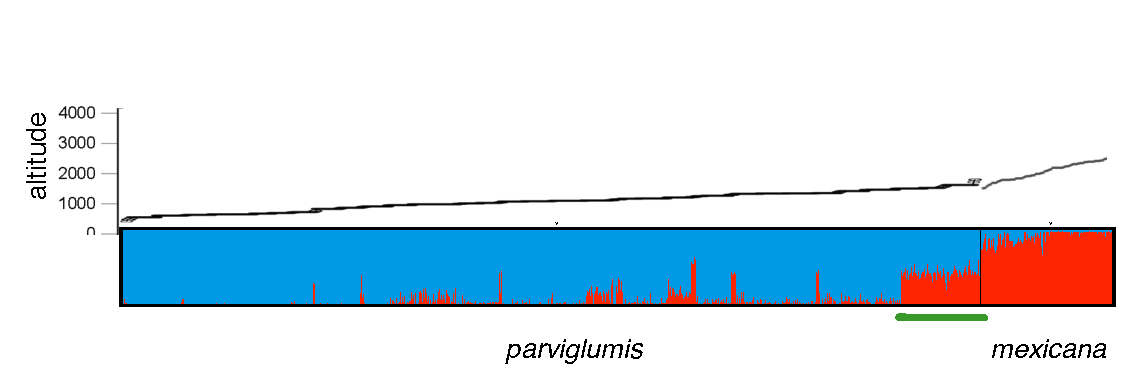
\includegraphics[width=0.95\textwidth]{structure.pdf}
    \caption{Assignment of \emph{parviglumis} and \emph{mexicana} individuals to K=2 groups using the Bayesian assignment algorithm of STRUCTURE \citep{Pritchard2000}.  Individuals are sorted by increasing altitude as indicated by the plot above the bar chart. Individuals from mid-elevation, hybrid zone populations are underscored in green.} 
\label{fig:structure}
\end{figure}

\begin{figure}[h!]
  \centering
   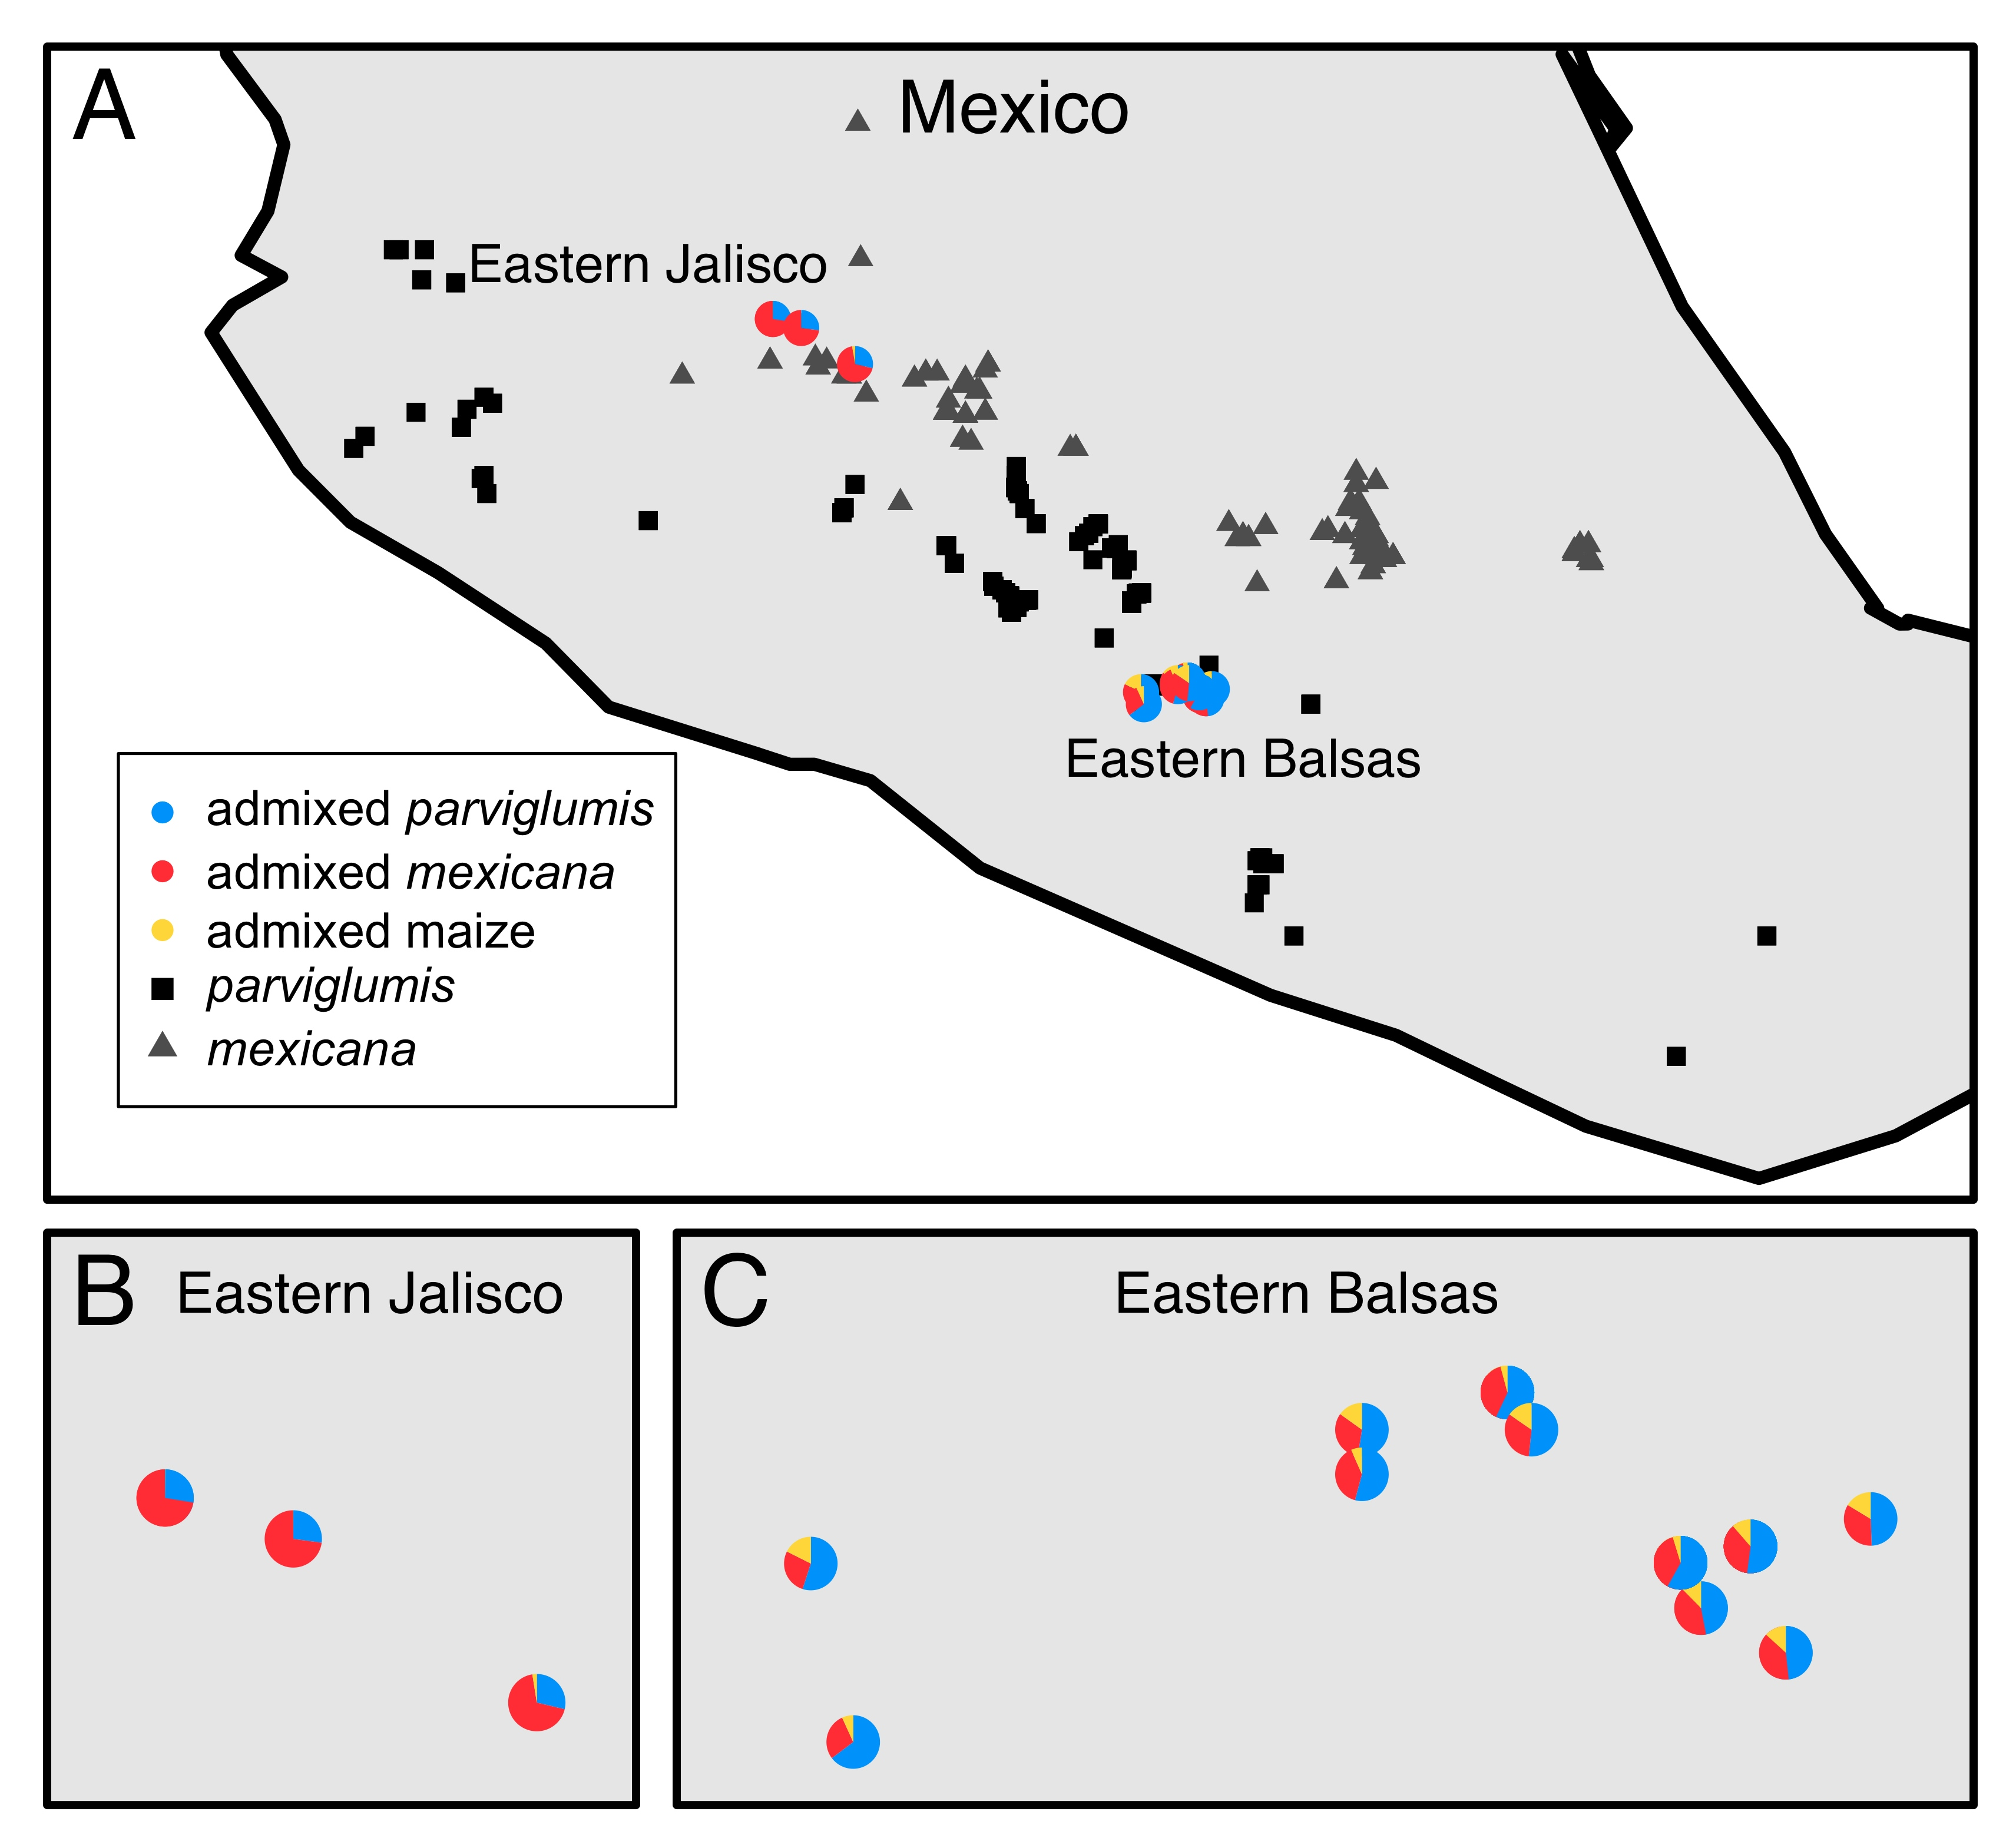
\includegraphics[width=0.7\textwidth]{Figure1.jpg}
    \caption{A) Location of two putative hybrid zones of \emph{mexicana} and \emph{parviglumis}.  Hybrid populations are represented as pie charts with proportion assigned to \emph{mexicana}, \emph{parviglumis}, and maize groups. Zoomed-in views of the Eastern Jalisco (B) and Eastern Balsas (C) hybrid populations.} 
\label{fig:pies}
\end{figure}
%
%\begin{table}[h!]
%\rowcolors{2}{gray!25}{white}
%\begin{center}
%\caption{Pairwise $F_{ST}$ between teosinte and hybrid populations} \label{tab:Fst}
%\begin{tabular}{lcccc}\\\toprule
%{\bf Taxon}&{\bf \emph{parviglumis}}&{\bf \emph{mexicana}}&{\bf Jalisco Hybrids}&{\bf Balsas Hybrids}\\\midrule
%{\bf \emph{parviglumis}}&---&---&---&---\\
%{\bf \emph{mexicana}}&0.107&---&---&---\\
%{\bf Jalisco Hybrids}&0.059&0.064&---&---\\
%{\bf Balsas Hybrids}&0.057&0.074&0.034&---\\\bottomrule
%\end{tabular}
%\end{center}
%\end{table} 
%

Currently, few studies have dissected the genome-wide architecture of hybridization in replicate hybrid zones, and little is known therefore about the consistency in patterns of gene flow.
The Hufford Laboratory and Senior Personnel Luis Eguiarte will assess the genomic architecture and evidence for selection on introgression in two hybrid zones of \zm{} and \zp{} through population collections, generation of genotype and sequence data, and application of population genomic analyses appropriate to this question. \jri{when to use ``pop genomic'' vs ``genetic'' we should be consistent}

\paragraph{\emph{Panel Construction and Sample Collection:}}\jri{these sections may need to move up}
From previous collections, we have access to extensive sampling of \zm{} and \zp{}.
Moreover, Senior Personnel Luis Eguiarte and collaborator Salvador Montes-Hernandez (see attached letter of commitment) have recently collected altitudinal transects of \zp{} and \zm{} that extend through both hybrid zones targeted by our project \citep{Diez2013} and are  familiar with populations in this region.
Our current collections will likely be insufficient for both the genotyping and common garden activities we propose and we have therefore budgeted for a collection trip during the first year of the project.
We will collect from 15 sampling sites in each of 16 populations.
Sampling sites will be randomly stratified across the elevation gradient of each population.
At each sampling site we will collect as much seed as possible from each of five teosinte plants (in the wild, teosinte plants produce an average of $\sim 100$ seeds per plant \citep{wilkes1967teosinte}). 
We will also measure plant density, slope of the terrain, and canopy cover at each sampling site.  These data will be useful covariates for estimating any potential maternal effects in our common garden experiments.  Four populations will be sampled from both the eastern Jalisco and eastern Balsas hybrid zones.  To the extent possible, we will select hybrid populations in a stratified manner across the elevation gradient found in these regions. Four populations each will also be collected from non-admixed \emph{parviglumis} and \emph{mexicana}, with two populations of each taxon collected from regions proximate to both hybrid zones.  We have already obtained the requisite collection permits as well as permits for importing samples into the United States for genetic analysis. Following collection, samples will be sent to the lab of Dr. Eguiarte at the Universidad Nacional Aut\'{o}noma de M\'{e}xico (UNAM) for cold storage until common garden experiments are planted (see \ref{sss:fitness}).  During year two of our proposed project, leaf tissue will be collected from a single plant per sampling site ($n=240$) in our mid-elevation common garden (see \ref{sss:fitness}) at the 5-7 leaf stage, stored in silica, and shipped to Iowa State University for DNA isolations and subsequent genotyping and full-genome sequencing.\jri{FYI silica isn't best for GBS. if possible ship fresh. remind me to give you  sampling protocol for plates. will save you time to collect into plates directly in field}

\paragraph{\emph{Sample Genotyping and Sequencing:}}
DNA for genotyping will be isolated using a modified CTAB procedure \citep{Saghai-Maroof1984}. \jri{another FYI: CTAB sucks for WGS. fine for GBS though} For sample genotyping ($n=240$) we will utilize the services of the Genomic Diversity Facility at Cornell University to implement a reduced representation approach to next-generation sequencing called Genotyping By Sequencing (GBS; \citealt{Elshire2011}; see attached letter of commitment from Dr. Sharon Mitchell). To date, this method has been implemented to genotype tens of thousands of maize samples and a bioinformatics pipeline (TASSLE-GBS) has been constructed that allows for genotyping $\sim$1,000,000 SNPs in maize \citep{Glaubitz2014} using standard GBS data. 
We will multiplex only 48 individuals per lane (instead of the standard 384 used for inbred lines) to minimize missing data and errors in identifying heterozygous genotypes. 
Based on our experience with diverse maize and teosinte \citep[e.g.][]{Takuno15062015, mezmouk2014pattern}, even after filtering for missing data, GBS provides many more markers with minimal ascertainment bias at a fraction of the cost of other available technologies. 

In addition to GBS data, we will generate full-genome sequence through the Iowa State University DNA Facility for a single hybrid individual from each hybrid zone.  We will generate two lanes of Illumina HiSeq 150bp, paired-end data per individual.  
We have previous experience dealing with whole genome shotgun data \citep{Gore2009,Chia2012a,Hufford2012b,da2015origin}, and have recently developed and implemented an open-source pipeline for read-mapping and SNP calling (\url{https://github.com/RILAB/paap}) using the existing maize B73 reference genome. 

\paragraph{\emph{Population Genomic Analyses:}} 
We will assess the genome-wide patterns of ancestry using several approaches.  
First, standard measures of differentiation including $F_{ST}$, the proportion of shared and fixed variants, and relative levels of nucleotide diversity \citep{Geneva2014} will be calculated in sliding windows along the genome. 
Second, we will attempt to implement haplotype-based methods for detecting introgression \citep[\emph{e.g.},][]{price2009, lawson2012} that will effectively allow us to model chromosomes from hybrid populations as mosaics of allopatric reference populations of \emph{parviglumis} and \emph{mexicana}.  
Finally, if phasing genotypes \citep{scheet2006fast} proves difficult given high levels of missing data or heterozygous error, we will make use of software designed to estimate admixture from genotype-likelihoods calculated on low-coverage sequence data \citep{skotte2013estimating}. 
We have already designed pipelines to work with genotype-likelihoods (e.g. \url{https://github.com/arundurvasula/angsd-wrapper}) and can utilize these methods to calculate standard diversity statistics.  
We will evaluate excess of \emph{parviglumis} or \emph{mexicana} ancestry on a site-by-site basis across hybrid genomes at the population level and will determine whether patterns are conserved across populations within hybrid zones and between hybrid zones.  Chromosomal regions showing an excess of ancestry from one taxon in hybrid populations will be inspected for evidence of selection using a combination of site-frequency-, linkage-disequilibrium-, and population-differentiation-based methods \citep[reviewed in][]{Vitti2013}. Chromosomal regions showing strong evidence of selection across individuals within a hybrid zone based on analysis of GBS data will be inspected in our whole-genome resequencing data to refine haplotype boundaries. 
Whole genome sequence data will also allow estimation of the age of the introgression and potentially identification of candidate causal polymorphisms.

		

\paragraph{\emph{Preliminary Results:}} 
\jri{add here prelim growth chamber expers. that suggest hybrids better than parents in some pops.}

\paragraph{\emph{Potential Challenges:}}
\jri{add here that if field collects not work, we already have smaller sets of seed from hybrid pops collected by collabs}


\subsection{Determine the extent to which anthropogenic movement of maize has enabled hybridization among taxa in \emph{Zea}} \label{ss:genuswide}

Following its domestication from \zp{} maize spread rapidly across the Americas \citep{Piperno2001,Grobman2012}, colonizing novel environments distinct from that inhabited by its wild ancestor. 
As its range expanded, maize came into contact with other wild teosinte that had been allopatric to \zp{} for    long periods prior to domestication \citep{hufford2012inferences}.  
Hybridization between maize and each of these taxa has been documented based on morphological \citep{wilkes1967teosinte, Wilkes1977} and genetic \citep{doebley1990molecular,Fukunaga2005,Ross-Ibarra2009a,vanheerwaarden2011a} data, raising a number of questions about the role of gene flow in the recent evolution of both maize and its wild relatives.

In this objective, the Ross-Ibarra Laboratory will use population genetic approaches to address three questions that arise from this natural experiment.  
First, we use maize and teosinte populations in Guatemala to investigate whether divergence time between taxa affects the possibility of adaptive introgression. 
Second, we take advantage of multiple pairs of sympatric maize and teosinte populations from both Mexico and Guatemala to test hypotheses about the geographic scale of adaptive introgression.
Finally, we use population-level comparisons of maize and all the diploid taxa in \emph{Zea} to test the hypothesis that maize has served as a bridge for gene flow between otherwise allopatric teositne \citep{Ross-Ibarra2009a}.

%DIVERGENCE TIME%%%%%%%%%%%%%%%%%%%%%%%%%%%%%%%%%%%%%%%%%%%%%%%%%%%%%%%%%
\subsubsection{Do the fitness consequences of gene flow from locally adapted populations depend on divergence?}
\label{sss:adaptive_intro}

Most models of speciation predict that introgression between taxa should decrease with increasing divergence between them \citep{harrison2014hybridization}, as differences contributing to postzygotic isolation are expected to increase as the square of divergence time \citep{orr2001evolution}. Maize colonization of the tropical lowlands of Guatemala offers an opportunity to test the importance of divergence in restricting the potential for adaptive introgression.

Upon arrival in Guatemala, maize came into contact with the wild teosintes  \emph{Zea mays} ssp. \emph{huehuetenangensis} (hereafter, \emph{huehuetenangensis}) and \emph{Zea luxurians} (hereafter, \emph{luxurians}). 
Conditions in Guatemala are substantially more tropical than the southwest coast of Mexico inhabited by \zp, with warmer winters, lower annual fluctuation in temperature, and nearly double the annual precipitation.
Both teosinte exhibit a number of adaptations to their environment including differences in root architecture, flooding tolerance, and delayed flowering \citep{wilkes1967teosinte, mano2006}.
Hybrids between maize and both taxa \citep{wilkes1967teosinte} have been observed, providing the opportunity for adaptive introgression.  
If divergence impacts the potential for adaptive introgression, we predict different patterns of maize-teosinte hybridization for each of these taxa. Divergence time between maize and \zh{} is not known, but it has been classified as a subspecies of \emph{zea mays} \citep{doebley1990systematics} and we predict that adaptive introgression from \zh{} is likely, much as we have previously observed from \zm{} \citep{Hufford2013}.
\emph{Zea luxurians}, however, exhibits a number of morphological differences from \emph{Zea mays} \citep{doebley1980taxonomy}, has a much larger genome \citep{tenaillon2011genome}, and divergence time between the two taxa has been estimated at $\sim150,000$ generations \citep{Ross-Ibarra2009a}. We predict that there will be less overall evidence for introgression from \zl{} due to the increased likelihood of loci causing postzygotic isolation.  
If adaptive introgression is observed, we predict it will be at fewer loci due to potential linkage with other incompatibility factors.

\begin{SCfigure}[][t]
  \centering
   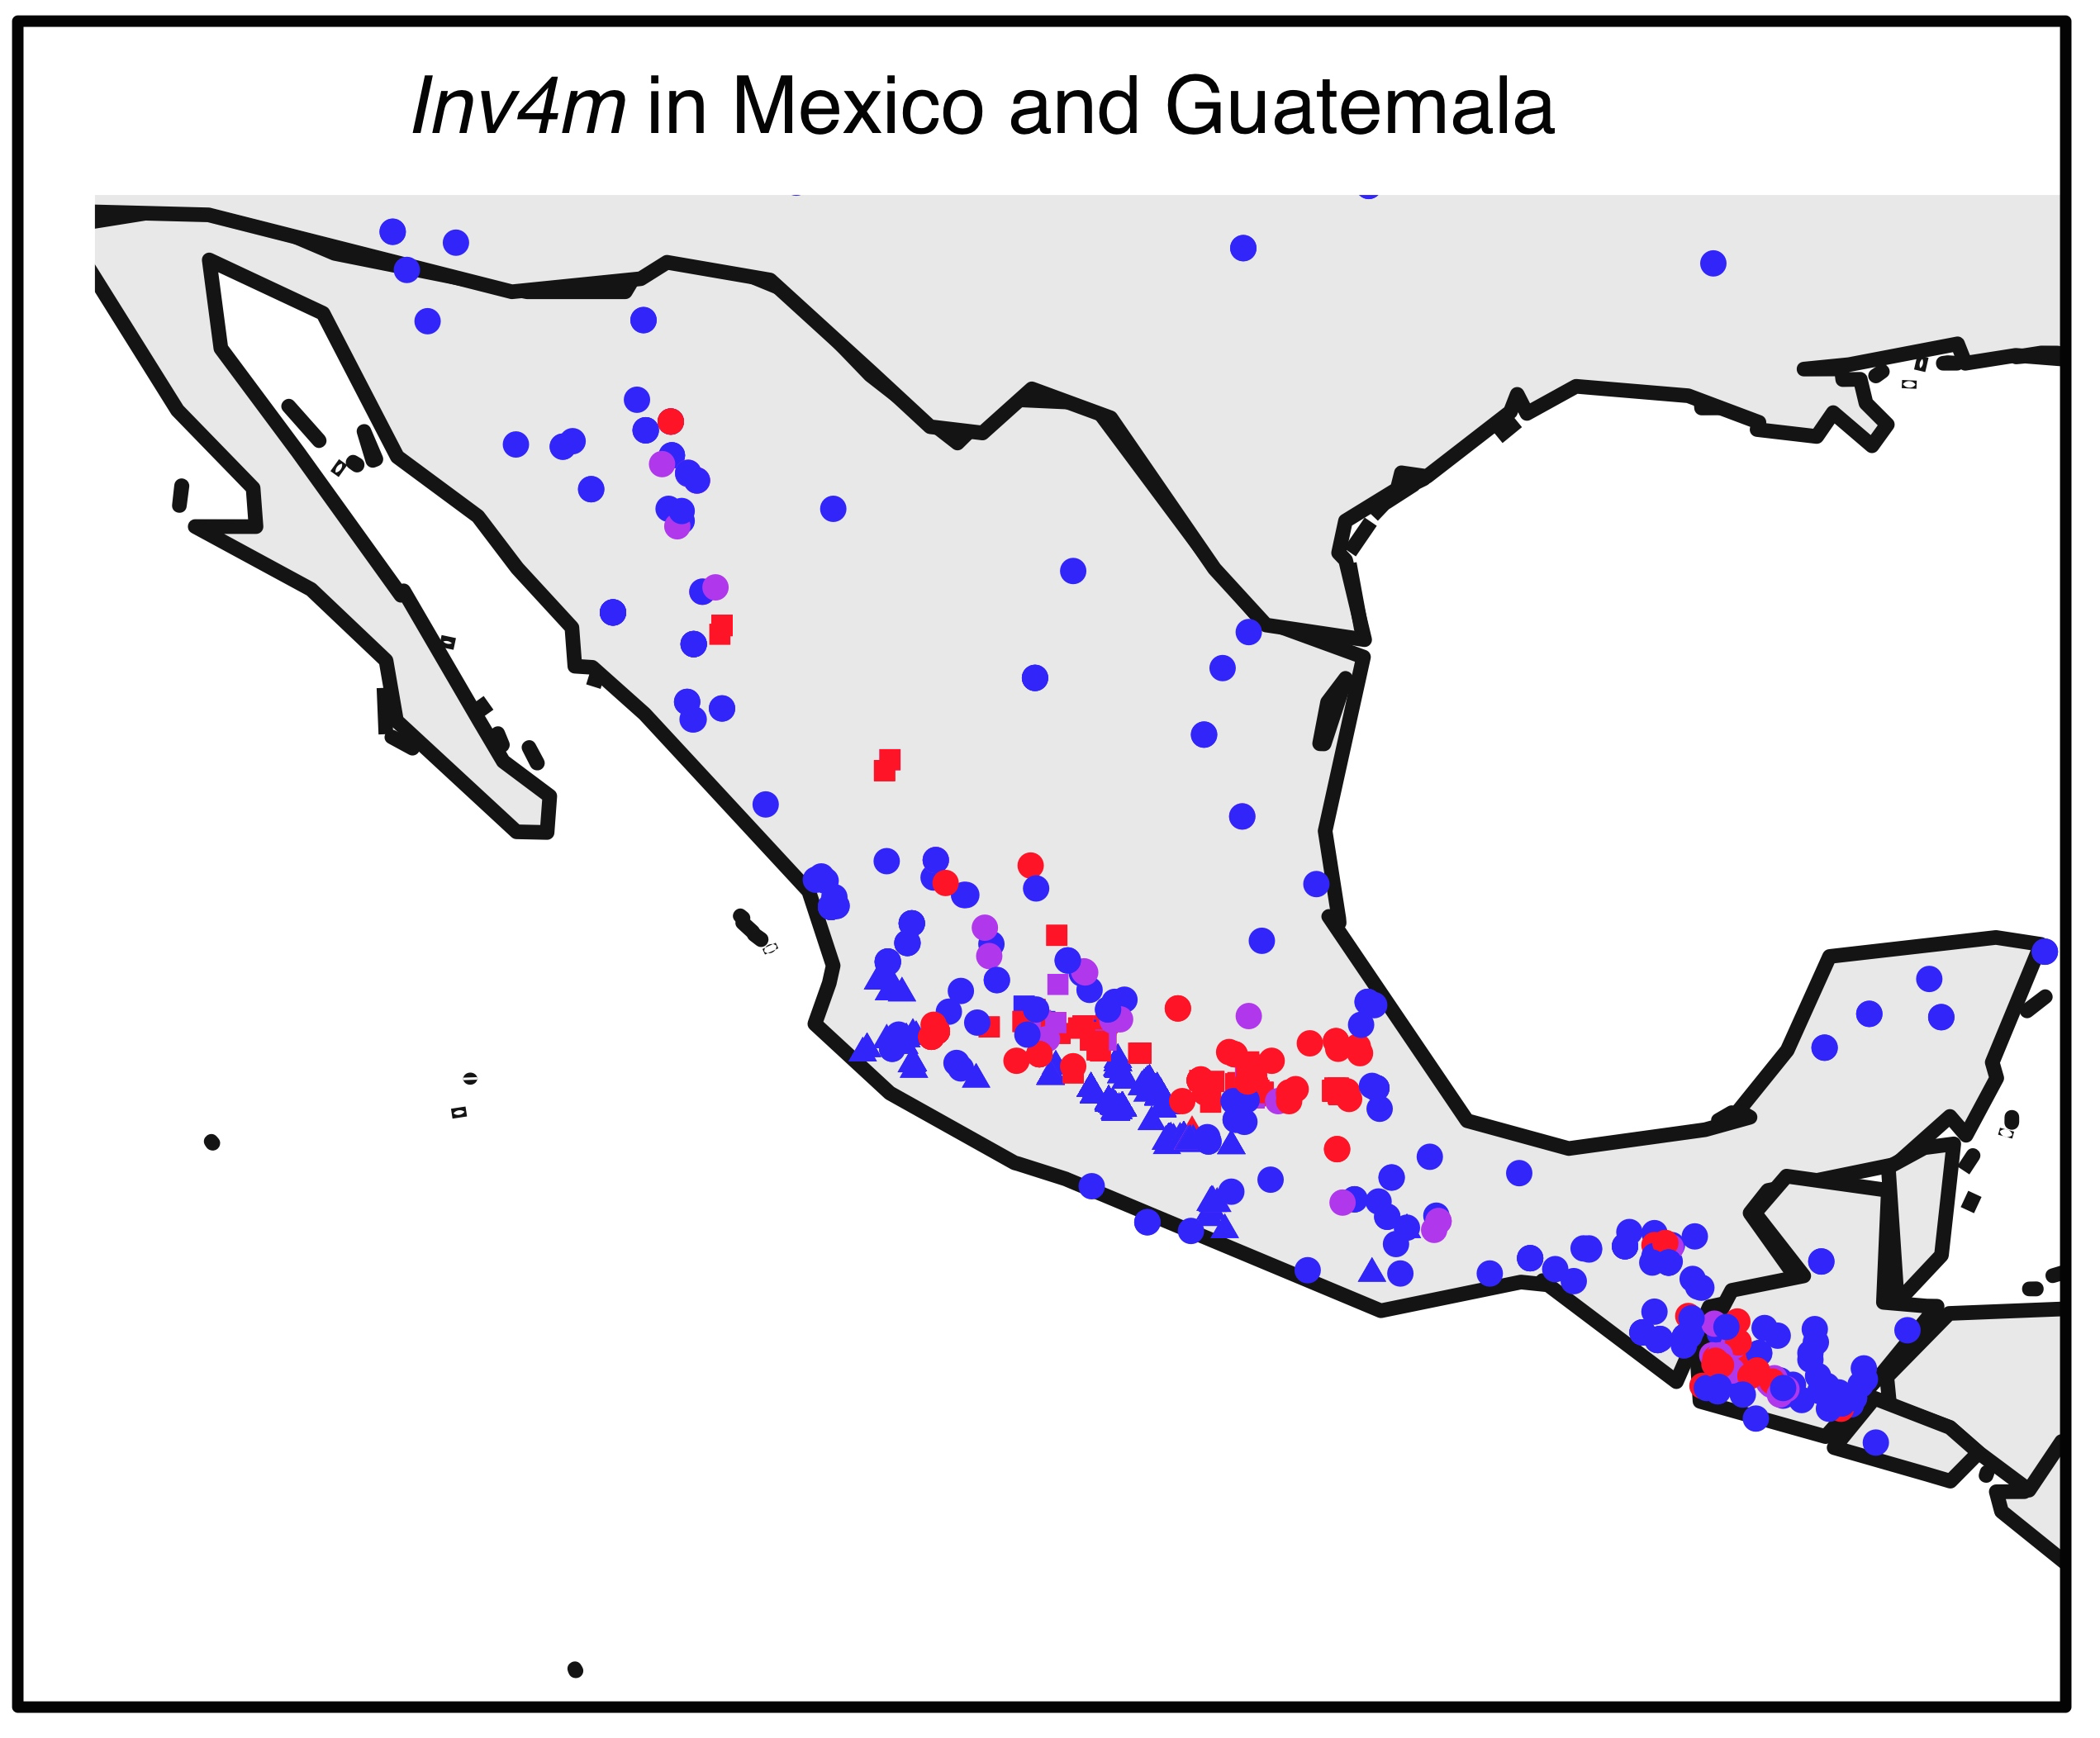
\includegraphics[width=0.5\textwidth]{inv4m_lux}
    \caption{ Geographic distribution of alleles at a SNP found to be diagnostic of the \emph{Inv4m} inversion.  Genotypes are shown in color (blue: homozygous standard, purple: heterozygous, red: homozygous inverted) and shapes represent taxa (squares: \zm, triangles: \zp, circles: domesticated maize)} 
\label{fig:inv4mmap}
\end{SCfigure} 
 \jri{need to cite this somewhere!}

To test  this question we will sample six populations of both \zl{} and \zh{}, stratified across their elevational range in Guatemala.  
Two of these populations will be chosen to be as distant as possible from domesticated maize, and used as a control representative of ancestral haplotypes or allele frequencies.  
For the remaining four populations of each taxon, we will sample populations of both the teosinte and a sympatric or nearby maize landrace population.
Additionally, two maize populations from similar environment, but allopatric to teosinte, will also be chosen, for a total of 24 maize and teosinte populations.
We will be assisted in our collection efforts by Mario Fuentes L\'{o}pez of the Fundit Organization in Guatemala (see attached letter of commitment).
We will genotype 12 individuals from each population using GBS. 
Two individuals (either two \zl\ or one \zl\ and one maize) will be fully sequenced.
There is currently no full genome sequence of \zl, and this will allow us to delineate introgressed or selected regions, identify copy number variants, and potentially identify candidate adaptive polymorphisms within the regions of interest.
Analysis of introgression and selection will follow methods described in \ref{sss:genomescan}.
If introgression from either of these teosintes has been adaptive to colonization of Guatemala, we predict we will find evidence of introgression in the majority of maize populations, that these regions will show evidence of recent selection in maize, and that they will overlap with QTL for phenotypes likely to be adaptive in these environments \citep[e.g.][]{omori2007qtl,mano2008linkage}.
We also predict that the same regions should show evidence of selection against introgression from maize into \zl.
Results from these analyses will help establish whether observations of adaptive introgression from \zm{} are an anomaly unique to the highlands of Mexico, or whether adaptive introgression from crop wild relatives may be a common occurrence that has facilitated the spread of domesticated taxa beyond their original habitat.

Finally, this aim will also provide useful baseline information on patterns of genetic diversity in \zl{} and \zh, both taxa of conservation concern within Guatemala and of interest for novel root phenotypes for breeding including root angle, adventitious root formation, and the formation of aerenchyma \citep{omori2007qtl,mano2007breeding}. 
Almost nothing is known about diversity in these taxa, and questions regarding their evolutionary history, long-term survival, the risk of diversity loss or extinction due to excessive hybridization with maize, and the relationship and connectivity among populations will all be furthered by the results obtained here.


%SPATIAL SCALES%%%%%%%%%%%%%%%%%%%%%%%%%%%%%%%%%%%%%%%%%%%%%%%%%%%%%%%%%
\subsubsection{Is introgression adaptive across multiple spatial scales?}
\label{sss:scale}


\begin{figure}[t]
  \centering
   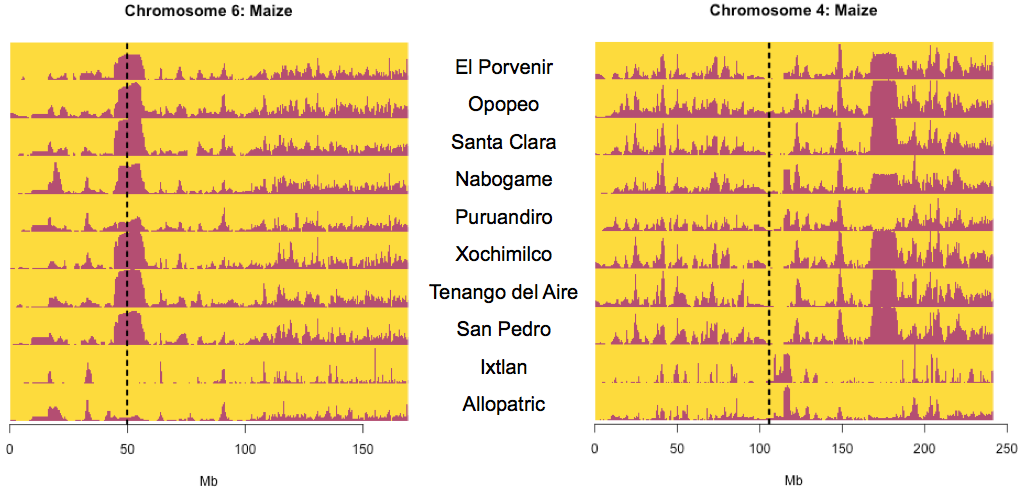
\includegraphics[width=0.75\textwidth]{same_regions}
    \caption{ Introgression from \zm\ to maize along chromosomes 4 and 6 \citep{Hufford2013}. Each row represents a population of maize, and the frequency of the \zm\ allele at a given position is shown in dark red. The strong signal of introgression at Mb 170 on chromosome 4 is the inversion polymorphism \emph{Inv4m}.} 
\label{fig:sameregions}
\end{figure} 



 In the  found consistent patterns introgression into several highland maize populations at QTL for phenotypes (\emph{e.g.}, pigment and macrohairs) that distinguish highland \zm{} from lowland \zp{} teosinte, and showed that both \zm{} phenotypes and higher growth rate were found in maize plants with \zm{}  introgression \citep{Hufford2013}.

Due to their sessile nature, plants must adapt to their local environments. 
The scale of local adaptation varies widely, from large geographic regions \citep{lowry2010, fang2014} to fine scale adaptation within a population \citep{hamrick1979}.  
While there are now several example of introgression facilitating adaptation in plant populations, we know little about the geographic scale at which this occurs.
Alleles that have spread throughout a wide geographic range in local populations have been tested in multiple genetic backgrounds and multiple microenvironments, and as such may have a higher likelihood of being adaptive in new populations via introgression.
In contrast, the selective benefit of alleles that have are adaptive on a local scale in a single population may depend more strongly on genetic background or particular aspects of the microenvironment and may fare worse when introgressed into a new population. 

We observed widespread introgression of \zm{} alleles in highland maize across the Central Plateau \citep{Hufford2013}, suggesting that some \zm{} alleles increased the fitness of maize across a wide geographic area.  
We also observed a number of introgressed regions at high frequency in only one or a few of the sympatric maize populations, suggestive of introgression
Unfortunately our previous SNP data provides poor resolution to identify selection \citep{tiffin2014advances} and suffers from ascertainment bias that limits detection of \zm\ haplotypes \citep{Hufford2013}.  

To understand the scale of adaptive introgression and local adaptation in maize, we propose here to analyze a set of sympatric pairs of maize and teosinte populations from the highlands of Central Mexico (with \zm), the Pacific coast of Mexico (with \zp), and the humid lowlands of Guatemala (with \zl\ and \zh). 
In addition to re-analysis of the populations sampled in \ref{sss:adaptive_intro}, we will sample three pairs of \zm\ and \zp\ previously identified as sympatric with domesticated maize \citep{hufford2010genetic, Hufford2013}.  
For each of \zl, \zm, \zp, and \zh\ we will endeavor to sample populations from different environments within the range of the taxon.
Maize and teosinte individuals from each population will be genotyped using GBS, and we will test for introgression and selection following methods proposed in \ref{sss:genomescan}.
Based on these results we will select two individuals (of maize or \zm) for whole-genome shotgun sequencing. 
The improved resolution offered by whole genome sequence will allow us to better characterize introgressed haplotypes and identify potential candidate loci.
We will quantify the overlap between regions of the genome showing evidence for selection and those showing evidence of introgression in all or a subset of sympatric populations.  
While we have prior evidence for adaptive introgression from \zm\ into maize, we do not know whether introgression from \zp, \zl, or \zh\ may have proven adaptive in any population.
If we find evidence of both introgression and selection, one hypothesis is that we may expect to find adaptive introgression limited to only those regions which are broadly adaptive across a wide geographic area. 
In this model, introgression may have been important for initial colonization of a new geographical area, such as the high altitudes of the Central Plateau, but continual gene flow from sympatric populations is selected against by farmers as it includes numerous deleterious alleles at domestication-related loci \citep[c.f.][]{Hufford2013}.
Alternatively, because there is considerable environmental variation even within a geographic area such as the Central Plateau \citep{hufford2012inferences, Pyhajarvi2013}, we may observe evidence for substantial adaptive introgression in localized pairs of populations, with little overlap among populations. 
Under this model, adaptive introgression not only allows colonization of new regions, but also better adapts maize to local conditions.


%BRIDGE%%%%%%%%%%%%%%%%%%%%%%%%%%%%%%%%%%%%%%%%%%%%%%%%%%%%%%%%%
\subsubsection{Can a widespread species serve as a bridge for introgression among allopatric species?}
\label{sss:bridge}

Additionally, based on analysis of a small number of resequenced loci, \emph{mexicana} haplotypes appear to be segregating in \emph{luxurians} \citep{Ross-Ibarra2009a}.  
Since \emph{mexicana} and \emph{luxurians} are entirely allopatric in their distributions, this suggests maize may have served as a bridge for gene flow between these two taxa.  
Further work will be necessary to explore this possibility and to assess if the genomes of \emph{Zea} species have been largely altered through gene flow during the spread of maize across the Americas (see \ref{ss:genuswide}).

Finally, we return to the observation of haplotype sharing between allopatric teosinte taxa \citep{Ross-Ibarra2009a} and propose to test whether these results are best explained by incomplete lineage sorting or the possibility that domesticated maize may have served as a bridge for indirect gene flow among teosinte populations. 

Population structure  initial survey of divergence and gene flow in \emph{Zea}, based on a set of 26 Sanger-sequenced loci, found evidence for admixture between allopatric populations of \emph{mexicana} and \emph{luxurians} at multiple loci \citep{Ross-Ibarra2009a}. 
As there is no evidence to suggest that these populations overlapped in their recent history, we took these results to suggest that maize, which is known to hybridize with both taxa, may have served as a bridge for gene flow between them.
Further support for this idea comes from patterns of haplotype segregation at an inversion locus on chromosome 4 \citep[\emph{Inv4m};][]{Fang2012,Pyhajarvi2013,Hufford2013}. 
The inverted haplotype at this locus appears to be derived in \emph{mexicana} \citep{Pyhajarvi2013}, but has introgressed into maize in the highlands of Mexico, an apparent example of adaptive introgression \citep[Panel A, Figure \ref{fig:hufmap};][]{Hufford2013}.
We have screened the $>2000$ samples in this data set for a SNP diagnostic for the inverted \emph{mexicana} haplotype and have found that the \emph{mexicana} haplotype is segregating in maize in the highlands of both Mexico and Guatemala (Panel B, Figure \ref{fig:hufmap}).  The haplotype is also present in all samples of \emph{luxurians} genotyped in \citet{Fang2012}.
These preliminary results suggest that the inversion has moved from \emph{mexicana} into \emph{luxurians}, perhaps via a maize intermediate.

\begin{figure}[]
  \centering
   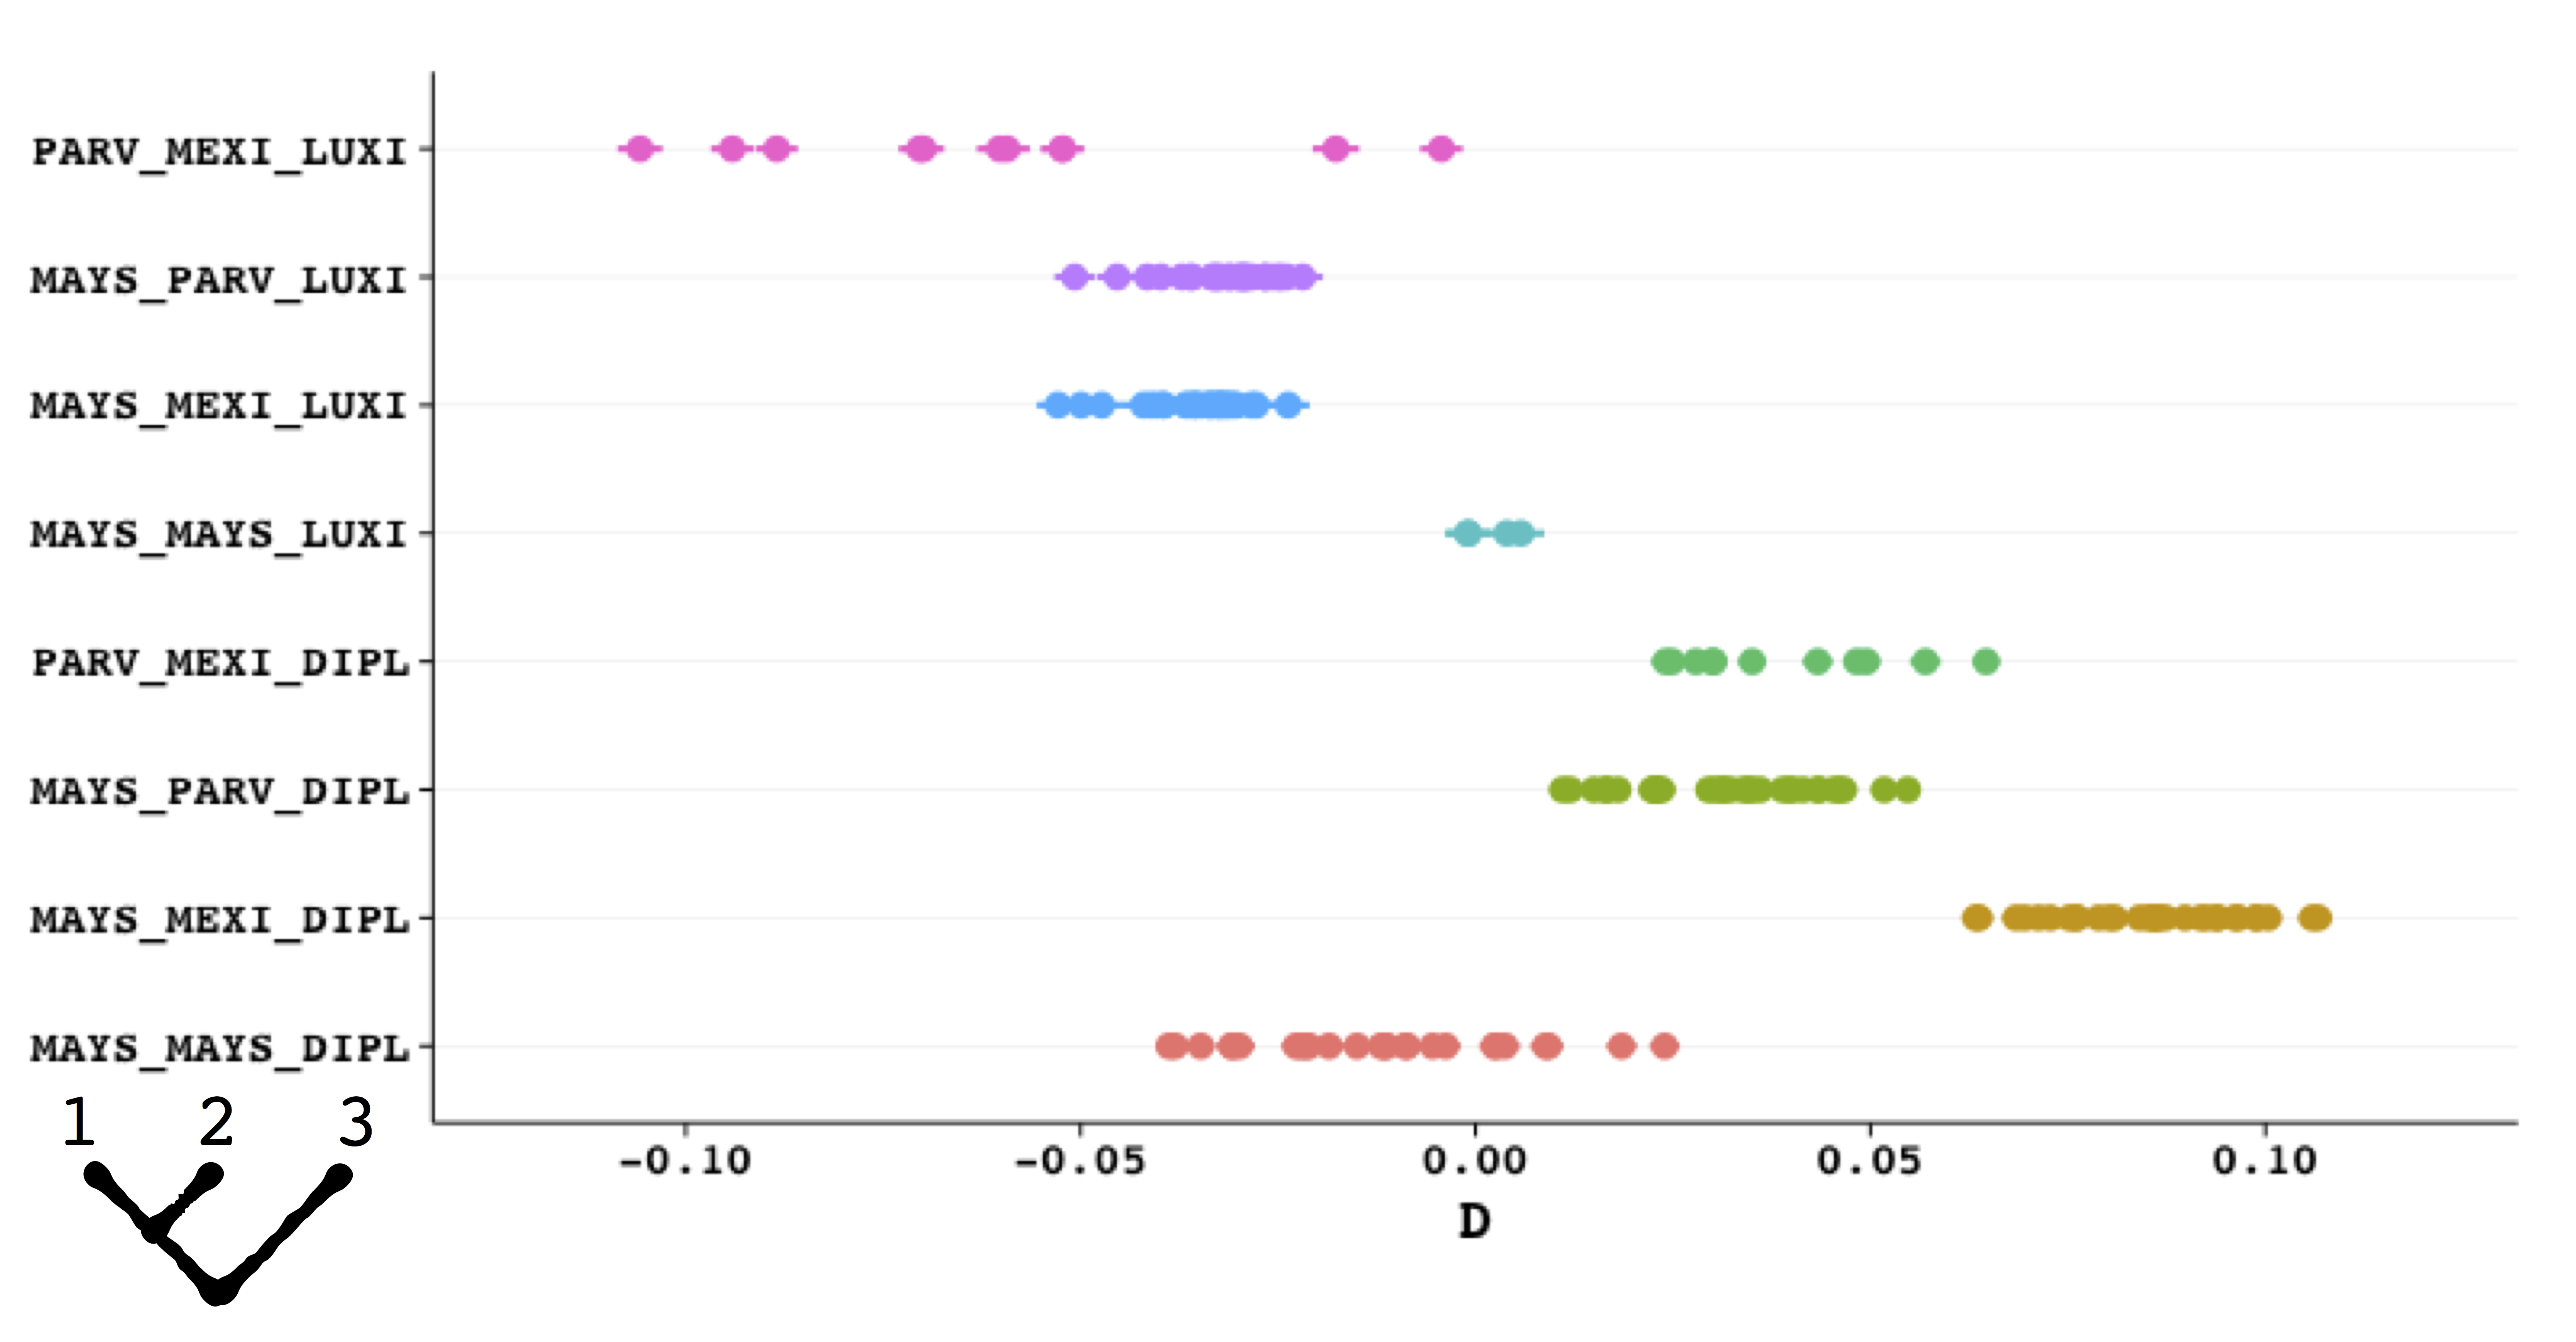
\includegraphics[width=0.8\textwidth]{abbas}
    \caption{Genome-wide evidence for admixture among \emph{Zea}. In the absence of admixture, taxa 1 and 2 on the tree shown should share similar numbers of derived alleles with taxa 3 due to incomplete lineage sorting.  Admixture leads to deviations from this expectation as measured by the D statistic  \citep{green2010draft}. Negative values of D indicate admixture between taxa 1 and 3, while positive values indicate admixture between taxa 2 and 3.} 
\label{fig:abba}
\end{figure}


Our preliminary analyses identified shared haplotypes in allopatric teosinte taxa, suggesting that maize may have served as a bridge for gene flow between \emph{mexicana} and \emph{luxurians} and potentially other \emph{Zea} taxa (see above).  However, an alternative explanation is that these loci were polymorphic in a common ancestor and continue to segregate due to incomplete lineage sorting.
Simple estimates of the length of shared haplotypes expected to be unbroken by recombination suggest that, over the $\sim 140,000$-generation divergence time between \emph{mexicana} and \emph{luxurians} \citep{Ross-Ibarra2009a}, we might well expect to see shared haplotypes of even several kb in length in low recombination regions of the genome (Figure \ref{fig:length}).
The high-density, genome-wide data generated here will provide an opportunity to test whether observed patterns of haplotype sharing between previously allopatric \emph{Zea} are due to recent introgression from maize.  
If shared haplotypes have come from introgression from maize over the last few thousand years, the genome-wide distribution of shared haplotype lengths should reveal longer shared segments (Figure \ref{fig:length}) than if haplotype sharing is due to incomplete lineage sorting alone.

No high-resolution genetic map currently exists for any teosinte, but the Ross-Ibarra group is currently working on producing such a map for \emph{parviglumis} as part of a different NSF project (\# 1238014), and evidence from comparisons among maize populations finds remarkable stability of the genetic map at a relatively coarse scale \citep{bauer2013} suggesting differences in the genetic map are unlikely to dramatically affect our estimates. 
Will will use our teosinte genetic map or the published NAM map \citep{McMullen2009} to generate an expected distribution of shared haplotype lengths along the genome based on expected divergence times between taxa.

Although the limited sampling in \citet{Ross-Ibarra2009a} only identified shared haplotypes between \zm\ and \zl, maize has been found to hybridize with all species in \emph{Zea} \citep{Wilkes1977}.
We will thus include in our analysis here the perennial taxa \emph{Zea diploperennis} (hereafter, \emph{diploperennis}) and \emph{Zea perennis} (hereafter, \emph{perennis}).  
We will sample 12 individuals from each of two populations of \emph{diploperennis} and \emph{perennis} and genotype these using GBS.
These populations, combined with samples from other teosinte populations included in \ref{sss:adaptive_intro} and \ref{sss:scale}, will provide us with a representative sample of wild teosinte populations from across the Americas.
Shared haplotypes will be identified (see methods in \ref{sss:genomescan}) and compared to the expected distribution of haplotype lengths to look for evidence of recent introgression consistent with the hypothesis that maize has served as a bridge for gene flow among teosinte taxa.
Although we cannot exhaustively test for the presence of such haplotypes in all of maize, we can survey published GBS data for more than $>16,000$ maize samples (\url{www.panzea.org}) to assess the frequency of such haplotypes in domesticated maize.

\subsubsection{Preliminary Results}
We have made arrangements with collaborators to assist in collection of maize, \zl\ and \zh\ from Guatemala.  The Ross-Ibarra and Hufford labs already have sufficient seed for all other samples for \ref{sss:bridge} and \ref{sss:scale}.
\jri{need more here}

\subsubsection{Potential Challenges}
\jri{need more here}


\section*{Broader Impacts}

Our efforts to broaden the impact of the research proposed here will begin within our groups through our commitment to effectively mentor volunteer undergraduate interns as well as graduate students and/or postdoctoral scholars funded by the project. Students and postdocs will receive one-on-one training from the investigators and senior personnel on laboratory, computational, and field research methods.  Mentees will also be encouraged and funded to present their work at scientific conferences.  Our groups have an excellent mentoring track record with four undergraduate students in the last five years publishing their work in scholarly journals and multiple underrepresented minorities participating in our research.

\jri{add something about undergraduate researchers in my lab?}

%\subsection*{ISU GK12 Fellowship Program}
%	
%In addition to the student and postdoc mentoring that will occur within our groups, as part of our broader impact activities each year one of our graduate students will participate in Iowa State University's GK12 Fellowship program (\emph{Symbi}; \url{http://www.gk12.iastate.edu/default.asp}; see attached letter of commitment). The selected graduate student will spend one full day each week in a middle or high school science classroom for the entire academic year of the Des Moines Public School District. This is the largest and most diverse school district in Iowa with over 50\% underrepresented minority student enrollment and over 70\% of students receiving free or reduced-cost lunch. The graduate student will introduce the K12 students to the scientific process through inquiry-based activities, relate the students’ science curriculum to real world examples, work with students on their science fair projects, and serve as a role model in a STEM profession. Furthermore, the graduate student will introduce students to his/her research project on hybridization and introgression in \emph{Zea}, a topic that is particularly well suited for teaching evolution in Iowa given the important role that maize plays in the Iowan economy. In introducing his/her dissertation research, the graduate student will engage Des Moines students in how research is conducted and provide STEM content professional training to his/her partner teacher.
%
%The GK12 Fellow will work with approximately 150 students on a regular weekly basis.  Student assessments from the ISU GK12 Fellowship Program have shown that a significant number of students like science more after having a GK Fellow in the classroom.  Teachers report that having a GK12 Fellow in their classroom is excellent professional development.  The PI will also visit the classroom and will support the selected graduate student in their development of appropriate material for the K12 audience.

\subsection*{US-Mexico Exchange Program}
	
Finally, we will establish a student exchange program between the Eguiarte Laboratory at UNAM in Mexico and the Hufford and Ross-Ibarra Laboratories in the United States. The Ross-Ibarra Laboratory has run an NSF-supported, US-Mexico exchange program for the last four years.  All of the exchange students involved in the program have continued on to additional graduate work, and two have earned authorship on forthcoming papers from their internship.  We will build upon the success of this program.  A student from the Eguiarte group will spend 2-3 months in either the Hufford or Ross-Ibarra Laboratory learning the GBS methodology and/or honing his/her skills in population genomic analysis, whereas a student from the Hufford and/or Ross-Ibarra Laboratories will travel to Mexico to participate in sample collection trips and to obtain expertise in common garden field experiments. This exchange will build capacity in all groups involved and will provide a valuable international research experience for a graduate student supported by the grant.  

Senior Personnel Claudia Calder\'{o}n has previously led international student research trips and will assist in preparing students from both the United States and Mexico for the exchange program. A survey will be given to both exchange students and faculty in order to gauge expectations prior to the trip and facilitate collaborations amongst the labs.  The survey will also assess students' knowledge and preconceived ideas  regarding their travel destinations.  A meeting (online or face-to-face) with the cohort of students traveling will help address these pre-conceptions and reduce cultural misunderstandings.  Suggestions will be given to students of how to prepare before the trip (visa, immigration requirements) and how to communicate with their peers and others during their exchange.  Students will be given information regarding the facilities where they will be staying, transportation to be used, food and water safety, the availability of telecommunications and general safety guidelines.

\required{Results From Prior NSF Support}
% 5 pages or fewer of the 15 pages for entire description document.
% include results from NSF grants received in the past 5 years.
% If supported by more than one grant, choose the most relevant one.

% For each grant, include: 
%	(a) NSF award number, amount, dates of support 
%	(b) The title of this project
%	(c) Publications resulting from this research
%	(d) Summary of the results of the completed work
%	(e) A brief description of data samples available and other research products not described 	      elsewhere
%	(f) For renewed support, a description of the relationship between the completed and 			      proposed work

% Due to space limitations, it is often advisable to use citations rather
% than putting the titles of the publications in the body 
% of this section

\subsection*{Hufford, Ross-Ibarra, Coop, Flint-Garcia, Sawers: \#1404974: US-Mexico Planning Visit and Workshop to Assess the Genomic Basis of Local Adaptation in Maize}
\$34,650. 09/01/14-08/31/15. PI Matthew Hufford, co-PIs J. Ross-Ibarra, G. Coop, Senior Personnel S. Flint-Garcia, Collaborators R. Sawers and A. Cibrian-Jaramillo
\par\noindent{\bf Intellectual merit} Through planning meetings and a phenotyping workshop in Mexico, this project has established a new international collaboration amongst principal investigators and laid the foundation for the work proposed in the current Plant Genome Research Program proposal. Planning meetings helped coordinate generation of preliminary data described in this proposal and the phenotyping workshop transferred high-throughput methods across our research groups.
\par\noindent{\bf Broader impacts}  Participants in the phenotyping workshop included graduate students and postdoctoral scholars from the United States and Mexico, providing STEM training and an international scientific experience.
\par\noindent{\bf Publications} Funding is for organizational purposes and generation of preliminary data; no publications have been produced under this award.

%\subsection*{Ross-Ibarra: \#1238014: Biology of Rare Alleles in Maize and Its Wild Relatives}
%\$13,311,185 (\$2,368,767 to Ross-Ibarra), 05/15/13-04/30/18. PI Edward Buckler, co-PIs J. Doebley, J. Holland, S. Flint-Garcia, Q. Sun, P. Bradbury, S. Mitchell, J. Ross-Ibarra
%\par\noindent{\bf Intellectual merit} In the first year we have developed accurate imputation approaches, found evidence for the importance of deleterious variants and non-genic polymorphisms in heterosis and GWAS, documented differences in recombination among the parents of the NAM population, and found population genetic evidence suggesting the importance of demography and purifying selection across the genome.  The grant has produced 18 total publications in its first year (only publications involving PIs Flint-Garcia and Ross-Ibarra are shown below).
%\par\noindent{\bf Broader impacts}  In the first year this project has included 10 postdoctoral and 12 graduate trainees. The GBS workshop and traveling maize exhibit continue to be popular and successful. A new version of the teacher-friendly guide to maize evolution has been revised and published online.
%\par\noindent{\bf Publications} \citet{peiffer2013genetic, Romay2013, wills2013many, Mezmouk2014, Peiffer2014, sood2014mining}

\subsection*{Ross-Ibarra: \#0922703: Functional Genomics of Maize Centromeres}
\$5,008,031 (\$754,409 to Ross-Ibarra). 09/01/09-08/31/14. PI Kelly Dawe, co-PIs J. Birchler, J. Jiang, G. Presting, J. Birchler, J. Ross-Ibarra
\par\noindent{\bf Intellectual merit} Centromeres are regions of the genome that organize and regulate chromosome movement, yet the biology of centromeres remains poorly understood. Co-PI Ross-Ibarra's group has focused in particular on the evolutionary genetics of centromeres. This work has demonstrated the remarkable evolutionary lability of centromere tandem repeats, but has shown that there is little evidence in maize for coevolution between centromere sequence and kinetochore proteins. Ongoing work from the Ross-Ibarra lab seeks to characterize kinetochore proteins, assess the phylogenetic evidence for longer-term coevolution, and understand patterns of centromere and genome size variation in natural populations.
\par\noindent{\bf Broader impacts}  Co-PI Ross-Ibarra has established an international student exchange program as part of this grant. Data and results of this project have been disseminated via publications and presentations as well as deposited in the maize genetics community database \url{www.maizegdb.org}. Former trainees on the grant include Dr. Matthew Hufford (PI on the current grant).\
\par\noindent{\bf Publications} \citet{Shi2010a, Chia2012a, Fang2012, Hufford2012, Hufford2012b, Hufford2013, Melters2013a, Kanizay2013, Pyhajarvi2013}